% Name: Filled contour plot
% Description: Level sets of a function of two variables, filled with a colormap, seen from above.
% Tags: contour, level sets, colormap, two variables

\usepackage{pgfplots}
\pgfplotsset{compat=1.18}

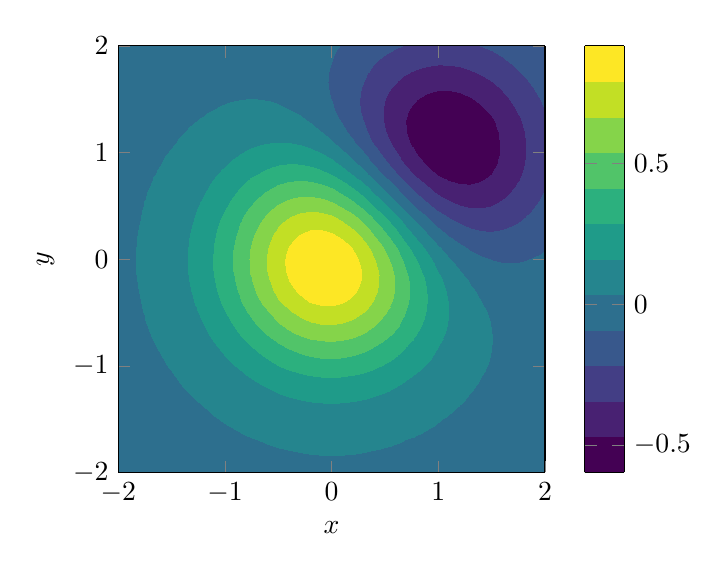
\begin{tikzpicture}
  \begin{axis}[
    view={0}{90}, width=8cm, height=7cm,
    xlabel=$x$, ylabel=$y$, colorbar, colormap/viridis,
    axis equal image, enlargelimits=false,
  ]
    \addplot3[contour filled={number=12}, domain=-2:2, domain y=-2:2, samples=41]
      {exp(-x^2 - y^2) - 0.7*exp(-(x - 1)^2 - (y - 1)^2)};
  \end{axis}
\end{tikzpicture}
